\documentclass[oneside,a4paper,14pt]{extarticle}
\usepackage[T1,T2A]{fontenc}
\usepackage[a4paper,letterpaper,top=20mm,bottom=20mm,left=25mm,right=15mm]{geometry}
\usepackage{amsmath, amssymb}
\usepackage[utf8]{inputenc}
\usepackage[russian]{babel}
\usepackage{textcomp}
\usepackage{indentfirst}
\usepackage{graphicx}
\usepackage{float}
\usepackage{mwe}
\usepackage{wrapfig}
\usepackage{caption}
\usepackage{tocloft}
\renewcommand{\cftsecleader}{\cftdotfill{\cftdotsep}}
\usepackage{longtable}
\usepackage{amsmath}
\usepackage{amsfonts}
\usepackage{amsthm}
\usepackage{float}
\usepackage[all]{xy}
\usepackage[breaklinks]{hyperref}
\usepackage{titlesec}
\usepackage{fancyvrb}
\usepackage{paracol}
\usepackage{minted}
\usepackage{xcolor}

\titleformat{\section}{\normalsize\bfseries}{\thesection}{1em}{}
\titleformat{\subsection}{\normalsize\bfseries}{\thesubsection}{1em}{}
\titleformat{\subsubsection}{\normalsize\bfseries}{\thesubsubsection}{1em}{}
\renewcommand\baselinestretch{1.33}\normalsize
\setlength{\parindent}{1.25cm}

\setlength{\emergencystretch}{3em}  % дополнительный запас для переносов

\begin{document}

\newpage\thispagestyle{empty}
\begin{center}
    МИНИСТЕРСТВО НАУКИ И ВЫСШЕГО ОБРАЗОВАНИЯ\\
    РОССИЙСКОЙ ФЕДЕРАЦИИ\\
    ФЕДЕРАЛЬНОЕ ГОСУДАРСТВЕННОЕ БЮДЖЕТНОЕ\\
    ОБРАЗОВАТЕЛЬНОЕ УЧРЕЖДЕНИЕ ВЫСШЕГО ОБРАЗОВАНИЯ\\
    ВЯТСКИЙ ГОСУДАРСТВЕННЫЙ УНИВЕРСИТЕТ\\
    Институт математики и информационных систем\\
    Факультет автоматики и вычислительной техники\\
    Кафедра электронных вычислительных машин
\end{center}

\vspace{20mm}
\begin{center}

    Отчёт по лабораторной работе №4\\
    по дисциплине\\
    Объектно-ориентированное программирование\\
\end{center}
\vfill

Выполнил студент гр. ИВТб-2301-05-00 \hfill
\makebox[8cm]{\hrulefill /Ковальский И.И./}

Проверил преподаватель\hfill
\makebox[8cm]{\hrulefill /Шмакова Н.А./}

\vfill
\begin{center}
    Киров\\
    2026
\end{center}

\newpage

\section*{Цель работы}
\addcontentsline{toc}{section}{Цель работы}
Разработка распределённого веб-приложения на языках Go и Python с использованием микросервисной архитектуры для реализации бизнес-логики и CRUD-операций над объектами согласованной предметной области. Доступ к существующей реляционной базе данных PostgreSQL осуществляется с использованием ORM SQLAlchemy.

\section*{Задание}
\addcontentsline{toc}{section}{Задание}

На основании согласованной в первой лабораторной работе предметной области «Организации» разработать распределённое веб-приложение, удовлетворяющее следующим требованиям:
\begin{enumerate}
    \item Использовать базу данных PostgreSQL, созданную в лабораторной работе №3. Структура БД, таблицы, связи и типы данных остаются без изменений.
    \item Реализовать сервер доступа к данным на языке Python (FastAPI + SQLAlchemy) с использованием паттерна Репозиторий. Модели должны точно соответствовать таблицам из ЛР №3 (включая \_\_tablename\_\_ и внешние ключи).
    \item Реализовать сервер бизнес-логики и отдачи веб-интерфейса на языке Go.
    \item На стороне Go реализовать: фильтрацию объектов, агрегацию (подсчёт суммы/количества), кэширование часто запрашиваемых данных (TTL 5 минут) и проверку бизнес-правил перед отправкой данных на Python-сервер.
    \item Реализовать веб-интерфейс (HTML/CSS/JS) с поддержкой всех CRUD-операций, валидацией, выпадающими списками для внешних ключей и отображением связанных сущностей.
\end{enumerate}

\newpage

\section*{Выполнение лабораторной работы}
\addcontentsline{toc}{section}{Выполнение лабораторной работы}

\subsection*{Архитектура распределённой системы}
\addcontentsline{toc}{subsection}{Архитектура распределённой системы}

Приложение построено по микросервисной архитектуре и разделено на две части:
\begin{itemize}
    \item \textbf{Go-сервер} (порт 8080) — сервер бизнес-логики и пользовательского интерфейса. Он принимает HTTP-запросы от браузера, выполняет валидацию, фильтрацию, агрегацию, кэширование, а затем через REST API обращается к Python-серверу для выполнения CRUD-операций над данными. Go-сервер также отвечает за генерацию HTML-страниц с помощью шаблонизатора.
    \item \textbf{Python-сервер} (порт 8000, FastAPI) — сервер доступа к данным. Он предоставляет REST API для работы с сущностями (коммерческие организации, некоммерческие организации, сотрудники). Python-сервер инкапсулирует всю логику взаимодействия с PostgreSQL и использует SQLAlchemy.
\end{itemize}

Связь между серверами осуществляется по протоколу HTTP: Go отправляет GET, POST, PUT, DELETE запросы на эндпоинты вида \texttt{/api/comorgs}, \texttt{/api/noncomorgs}, \texttt{/api/employees}. Python-сервер возвращает JSON-ответы, которые Go обрабатывает и передаёт в шаблоны.
\newpage
\textbf{Go запрашивает данные у python:}
\begin{small}

\begin{minted}{go}
    func indexHandler(w http.ResponseWriter, r *http.Request) {
	nameFilter := r.URL.Query().Get("nameFilter")
	minEmp, _ := strconv.Atoi(r.URL.Query().Get("minEmployees"))
	maxEmp, _ := strconv.Atoi(r.URL.Query().Get("maxEmployees"))
	sortEnabled := r.URL.Query().Get("sort") == "true"

	cd, _ := getFromCacheOrFetch(pythonAPI + "/api/comorgs")
	nd, _ := getFromCacheOrFetch(pythonAPI + "/api/noncomorgs")
	ed, _ := getFromCacheOrFetch(pythonAPI + "/api/employees")

	var comOrgs []ComOrg
	var nonComOrgs []NonComOrg
	var employees []Employee
	json.Unmarshal(cd, &comOrgs)
	json.Unmarshal(nd, &nonComOrgs)
	json.Unmarshal(ed, &employees)

	orgNameMap := make(map[int]string)
	for _, org := range comOrgs {
		orgNameMap[org.ID] = org.Name + " (Ком)"
	}
	for _, org := range nonComOrgs {
		orgNameMap[org.ID] = org.Name + " (Неком)"
	}

	for i := range employees {
		if name, ok := orgNameMap[employees[i].OrgID]; ok {
			employees[i].OrgName = name
		} else {
			employees[i].OrgName = ""
		}
	}

	var comOrgsDisplay []ComOrgDisplay
	for _, org := range comOrgs {
		empCount := countEmployees(employees, org.ID)
		comOrgsDisplay = append(comOrgsDisplay, ComOrgDisplay{
			ComOrg:         org,
			EmployeesCount: empCount,
			Taxes:          org.Taxes(),
		})
	}

	var nonComOrgsDisplay []NonComOrgDisplay
	for _, org := range nonComOrgs {
		empCount := countEmployees(employees, org.ID)
		nonComOrgsDisplay = append(nonComOrgsDisplay, NonComOrgDisplay{
			NonComOrg:      org,
			EmployeesCount: empCount,
			Taxes:          calculateNonComTax(empCount),
		})
	}
	filteredCom, filteredNon := filterOrgs(comOrgsDisplay, nonComOrgsDisplay, nameFilter, minEmp, maxEmp)

	var allOrgs []OrgOption
	for _, o := range comOrgs {
		allOrgs = append(allOrgs, OrgOption{ID: o.ID, Name: o.Name + " (Ком)"})
	}
	for _, o := range nonComOrgs {
		allOrgs = append(allOrgs, OrgOption{ID: o.ID, Name: o.Name + " (Неком)"})
	}
	sortedCom, sortedNon, sortedEmployees, sortedAllOrgs := sortByName(sortEnabled, filteredCom, filteredNon, employees, allOrgs)

	data := TemplateData{
		ComOrgs:      sortedCom,
		NonComOrgs:   sortedNon,
		Employees:    sortedEmployees,
		AllOrgs:      sortedAllOrgs,
		NameFilter:   nameFilter,
		MinEmployees: minEmp,
		MaxEmployees: maxEmp,
		SortEnabled:  sortEnabled,
	}

	tmpl := template.Must(template.ParseFiles("templates/index.html"))
	tmpl.Execute(w, data)
}
\end{minted}

\end{small}

\newpage

\textbf{Go отправляет данные в python:}
\begin{small}

\begin{minted}{python}
    func editHandler(w http.ResponseWriter, r *http.Request) {
	r.ParseForm()
	id := r.FormValue("id")
	orgType := r.FormValue("type")
	url := fmt.Sprintf("%s/api/%s/%s", pythonAPI, orgType, id)

	if orgType == "comorgs" {
		profit := r.FormValue("profit")
		if profitInt, err := strconv.Atoi(profit); err != nil || profitInt < 0 {
			profit = "0"
		}

		org := ComOrg{
			Name:         r.FormValue("name"),
			Inn:          r.FormValue("inn"),
			Profit:       profit,
			BusinessType: r.FormValue("businessType"),
		}
		requestJSON(http.MethodPut, url, org)
	} else if orgType == "noncomorgs" {
		org := NonComOrg{
			Name:    r.FormValue("name"),
			Inn:     r.FormValue("inn"),
			Purpose: r.FormValue("purpose"),
			Source:  r.FormValue("source"),
		}
		requestJSON(http.MethodPut, url, org)
	}
	invalidateCache()
	http.Redirect(w, r, "/", http.StatusSeeOther)
}
\end{minted}
\end{small}

\newpage
\subsection*{Файлы и классы проекта}
\addcontentsline{toc}{subsection}{Файлы и классы проекта}

Проект состоит из следующих файлов:

\paragraph{Файл main.go (Go-сервер)}
Содержит все структуры данных, бизнес-логику, обработчики HTTP-запросов, кэш и точку входа. В нём определены:

\begin{itemize}
    \item \textbf{Структура ComOrg} — коммерческая организация. Поля: ID, Name, Inn, Profit, BusinessType. Метод Taxes() вычисляет налог как 20\% от прибыли.
    \item \textbf{Структура NonComOrg} — некоммерческая организация. Поля: ID, Name, Inn, Purpose, Source.
    \item \textbf{Структура Employee} — сотрудник. Поля: ID, Name, Position, OrgID, OrgName (заполняется отдельно для отображения).
    \item \textbf{Структура OrgOption} — используется для выпадающих списков (ID + Name).
    \item \textbf{Структуры ComOrgDisplay и NonComOrgDisplay} — расширяют базовые типы, добавляя поля EmployeesCount и Taxes для отображения в таблицах.
    \item \textbf{Структура TemplateData} — данные, передаваемые в HTML-шаблон (списки организаций, сотрудников, параметры фильтрации).
    \item \textbf{Функции бизнес-логики}:
        \begin{itemize}
            \item countEmployees — агрегация: подсчёт числа сотрудников для организации.
            \item calculateNonComTax — расчёт налога для некоммерческой организации (10 рублей за каждого сотрудника).
            \item filterOrgs — фильтрация списков организаций по названию и диапазону численности сотрудников.
        \end{itemize}
    \item \textbf{Кэш с TTL 5 минут} — глобальные переменные cache и expiration, мьютекс cacheMutex, функции getFromCacheOrFetch и invalidateCache.
    \item \textbf{Обработчики HTTP}:
        \begin{itemize}
            \item indexHandler — главная страница: получает данные от Python, агрегирует, фильтрует, рендерит шаблон.
            \item getOrgHandler, editHandler, addComOrgHandler, addNonComOrgHandler — CRUD для организаций.
            \item getEmployeeHandler, editEmployeeHandler, addEmpHandler, deleteEmployeeHandler — CRUD для сотрудников.
            \item actionHandler — выполнение специфических бизнес-методов: expandBusiness (увеличить прибыль на 20\%) для коммерческих организаций и attractFunding (добавить источник финансирования) для некоммерческих.
            \item deleteHandler — удаление организаций.
        \end{itemize}
\end{itemize}

\newpage

\paragraph{Файл index.html}
HTML-шаблон, который использует Go-сервер для отображения интерфейса. В нём описаны:
\begin{itemize}
    \item Три таблицы: коммерческие организации, некоммерческие организации, сотрудники.
    \item Форма фильтрации (по названию и количеству сотрудников).
    \item Модальные окна для добавления и редактирования записей.
    \item JavaScript-функции для отправки бизнес-методов (submitActionForm, openParamModal) и динамической загрузки данных в модальные окна.
\end{itemize}

\paragraph{Файлы Python-сервера}
Сервер на Python состоит из:
\begin{itemize}
    \item \textbf{Модели SQLAlchemy}: Organization, ComOrg, NonComOrg, Employee. Они описывают таблицы и связи в БД.
    \item \textbf{Репозиторий} — класс с методами get\_all, get\_by\_id, create, update, delete. При изменении данных автоматически пересчитывает поле employees\_count в таблице organizations.
    \item \textbf{FastAPI-роуты} — эндпоинты /api/comorgs, /api/noncomorgs, /api/employees, а также /api/\{type\}/\{id\} для отдельных записей.
\end{itemize}

\begin{figure}
    \centering
    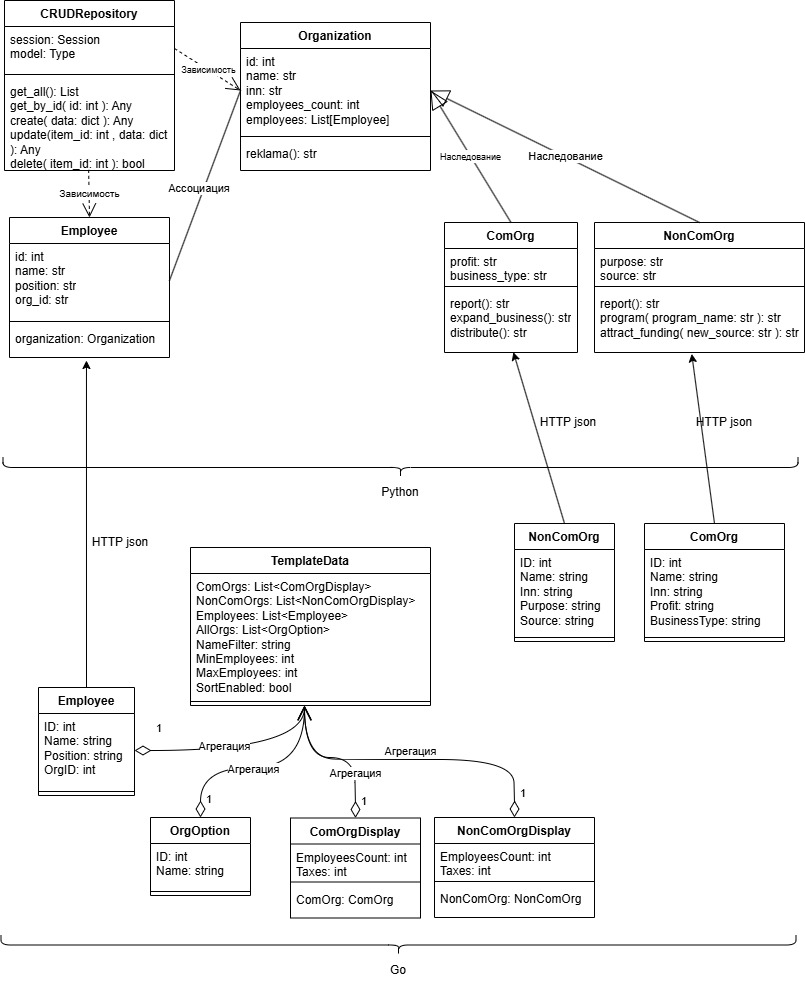
\includegraphics[width=0.9\linewidth]{Классы.jpg}
    \caption{Диаграмма классов}
    \label{fig:classes}
\end{figure}

\newpage

\subsection*{Слой доступа к данным}
\addcontentsline{toc}{subsection}{Слой доступа к данным}

Сервер на Python отвечает за непосредственное взаимодействие с базой данных PostgreSQL. Для описания структуры данных используется SQLAlchemy.

\begin{figure}[H]
  \centering
  
\includegraphics[width=0.8\textwidth]{ERD.png}
  \caption{ERD схема}
  \label{fig:ERD}
\end{figure}

\subsubsection*{Модели данных}

\textbf{Базовый класс Organization:}
Отображается на таблицу organizations. Содержит поля id, name, inn, employees\_count. Связь один-ко-многим с сотрудниками реализована через relationship "Employee", back\_populates="organization".

\textbf{Классы-наследники ComOrg и NonComOrg:}
Отображаются на таблицы comorganizations и noncomorganizations соответственно. Связь с родительской таблицей организована через внешний ключ organizations.id. Содержат специфичные поля: прибыль, тип бизнеса, цель, источник.

\textbf{Класс Employee:}
Отображается на таблицу employees. Содержит внешний ключ org\_id, ссылающийся на organizations.id с правилом ondelete="SET NULL".

\textbf{Пример модели данных:}
Python класс организации Organization
\begin{small}
    \begin{minted}{python}
    class Organization(Base):
    __tablename__ = "organizations"
    id = Column(Integer, primary_key=True, index=True)
    name = Column(String)
    inn = Column(String)
    employees_count = Column(Integer, default=0, nullable=False)

    employees = relationship(
        "Employee", back_populates="organization", cascade="all, delete-orphan"
    )

    __mapper_args__ = {
        'polymorphic_identity': 'organization',
        'polymorphic_on': None
    }

    def reklama(self):
        return f"{self.name} оч крутая!"
\end{minted}

\end{small}
Python класс сотрудника Employee:
\begin{small}
\begin{minted}{python}
    class Employee(Base):
    __tablename__ = "employees"
    id = Column(Integer, primary_key=True, index=True)
    name = Column(String)
    position = Column(String)
    org_id = Column(Integer, ForeignKey("organizations.id", ondelete="SET NULL"))

    organization = relationship("Organization", back_populates="employees")
\end{minted}

\end{small}

Go структура коммерческой организации ComOrg:
\begin{small}

\begin{minted}{python}
    type ComOrg struct {
    	ID           int    `json:"id"`
    	Name         string `json:"name"`
    	Inn          string `json:"inn"`
    	Profit       string `json:"profit"`
    	BusinessType string `json:"business_type"`
    }
\end{minted}
\end{small}


Go структура сотрудника Employee:
\begin{minted}{python}
    type Employee struct {
	ID       int    `json:"id"`
	Name     string `json:"name"`
	Position string `json:"position"`
	OrgID    int    `json:"org_id"`
	OrgName  string `json:"org_name"`
}
\end{minted}
\subsubsection*{Репозиторий}
\begin{itemize}
    \item get\_all() и get\_by\_id() — методы для чтения данных.
    \item create(), update(), delete() — методы для модификации данных.
\end{itemize}
\textbf{Особенность реализации бизнес-правил в БД:} При добавлении, обновлении организации или удалении сотрудника, репозиторий автоматически находит связанную организацию и обновляет поле employees\_count.

\subsection*{Слой бизнес-логики и представления}
\addcontentsline{toc}{subsection}{Слой бизнес-логики и представления}

Сервер на Go (файл main.go) реализует всю логику, не связанную напрямую с БД: валидацию, агрегацию, фильтрацию, кэширование и бизнес-методы. Он работает как HTTP-сервер на порту 8080 и предоставляет веб-интерфейс.

\subsubsection*{Бизнес-логика и агрегация}

Методы реализованы напрямую у структур Go:
\begin{itemize}
    \item \texttt{Taxes()} для \texttt{ComOrg}: высчитывает 20\% от прибыли. Преобразует строковое значение прибыли в число, валидирует отрицательные значения.
    \item \texttt{calculateNonComTax()}: рассчитывает налог для некоммерческих организаций как 10 рублей за каждого сотрудника.
    \item \texttt{countEmployees()}: агрегирующая функция, подсчитывающая точное количество сотрудников для конкретной организации на основе полного списка.
    \item \texttt{filterOrgs()}: осуществляет фильтрацию списка организаций по названию и по минимальному/максимальному количеству сотрудников.
\end{itemize}

\subsubsection*{Сортировка}

В текущей версии приложения явная сортировка данных не реализована, так как задание не предъявляет требований к сортировке. Таблицы отображают записи в том порядке, в котором их возвращает Python-сервер, а тот, в свою очередь, получает данные из PostgreSQL в порядке возрастания первичного ключа. Таким образом, организации и сотрудники выводятся стабильно по ID. При необходимости сортировку по любому полю (название, налог, количество сотрудников) можно легко добавить на стороне Go с использованием функции \texttt{sort.Slice}.

\subsubsection*{Обработчики HTTP}

\begin{itemize}
    \item \texttt{indexHandler}: Главный контроллер. Запрашивает данные у Python через кэширующую функцию, формирует map для быстрого поиска названий организаций, выполняет агрегацию (подсчёт сотрудников и налогов), применяет фильтры из параметров запроса, затем рендерит шаблон \texttt{index.html}.
    \item \texttt{editHandler}, \texttt{addComOrgHandler}, \texttt{addEmpHandler}: Собирают данные из HTML-форм, валидируют их (например, прибыль не может быть отрицательной) и отправляют POST/PUT запросы в Python в виде JSON.
    \item \texttt{actionHandler}: Реализует уникальные методы бизнес-логики. Например, \texttt{expandBusiness} (увеличивает прибыль коммерческой организации на 20\%) или \texttt{attractFunding} (добавляет новый источник финансирования в строку через запятую для некоммерческой организации). Перед отправкой изменений в Python выполняется проверка корректности параметров.
\end{itemize}

\subsection*{Веб-интерфейс}
\addcontentsline{toc}{subsection}{Веб-интерфейс}

Пользовательский интерфейс реализован с использованием стандартного пакета Go \texttt{html/template}. Ключевые особенности:
\begin{itemize}
    \item На главной странице расположены панели для фильтрации данных (поиск по имени, ограничение по числу сотрудников).
    \item Реализованы модальные окна или отдельные формы для создания и редактирования сущностей.
    \item При добавлении/редактировании сотрудника выбор организации осуществляется через выпадающий список (\texttt{<select>}), который динамически заполняется сервером (массив \texttt{AllOrgs}).
    \item В таблицах отображаются рассчитанные "на лету" данные: актуальное количество сотрудников и налоги, что демонстрирует работу слоя бизнес-логики.
    \item Добавлена клиентская валидация форм: отрицательные значения прибыли или количества сотрудников блокируются.
\end{itemize}

\newpage

\subsection*{Экранные формы}
\addcontentsline{toc}{subsection}{Экранные формы}

\begin{figure}[H]
  \centering
  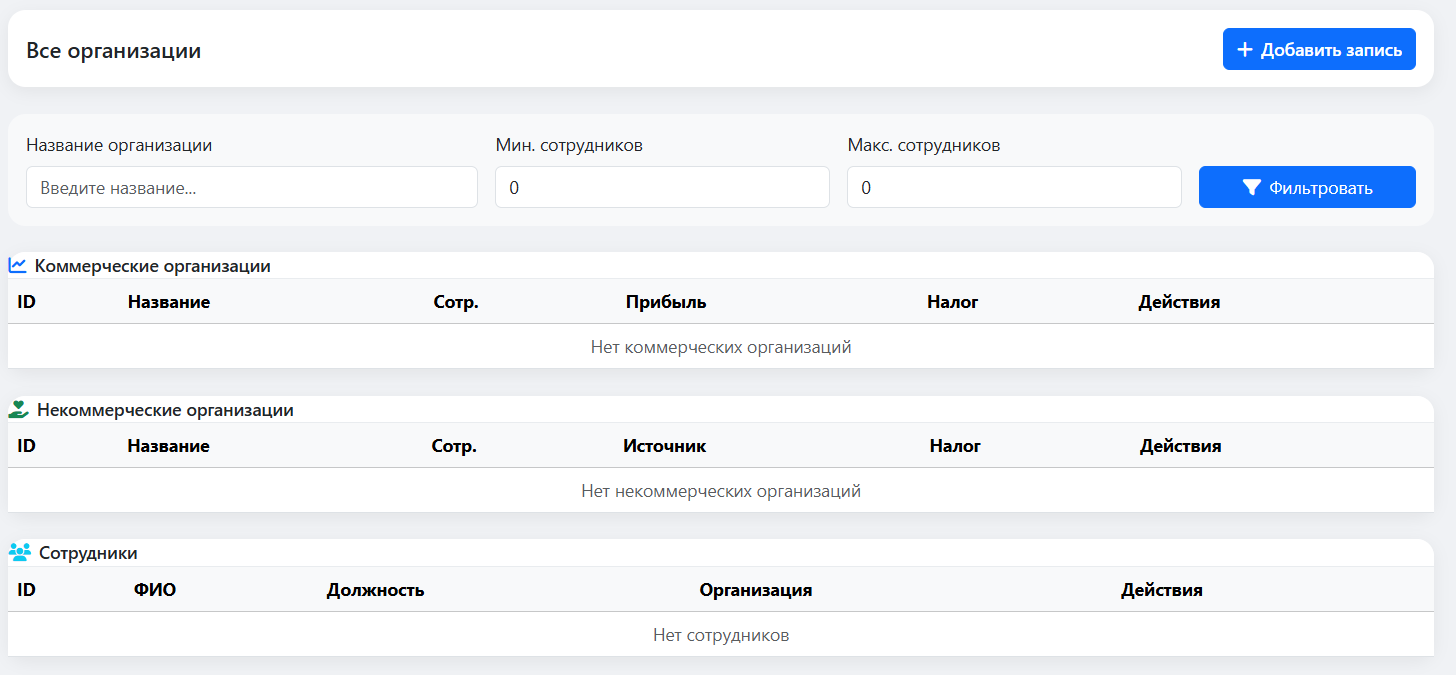
\includegraphics[width=0.9\textwidth]{главная.png}
  \caption{Главная страница}
  \label{fig:index_page}
\end{figure}


\begin{figure}[H]
  \centering
  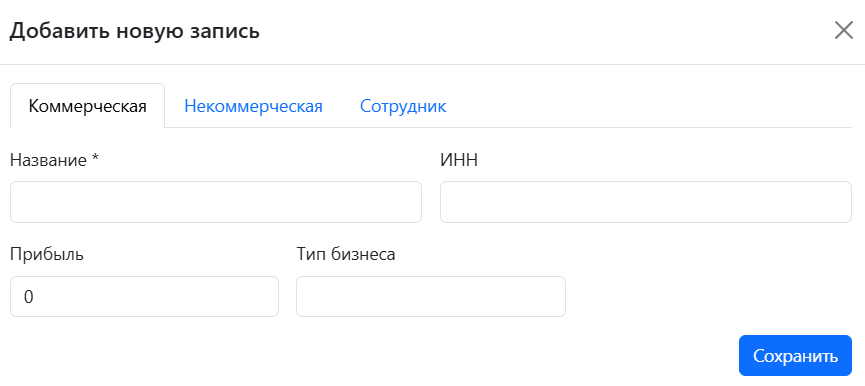
\includegraphics[width=0.8\textwidth]{добавление коморг.png}
  \caption{Форма добавления коммерческой организации}
  \label{fig:add_com}
\end{figure}


\begin{figure}[H]
  \centering
  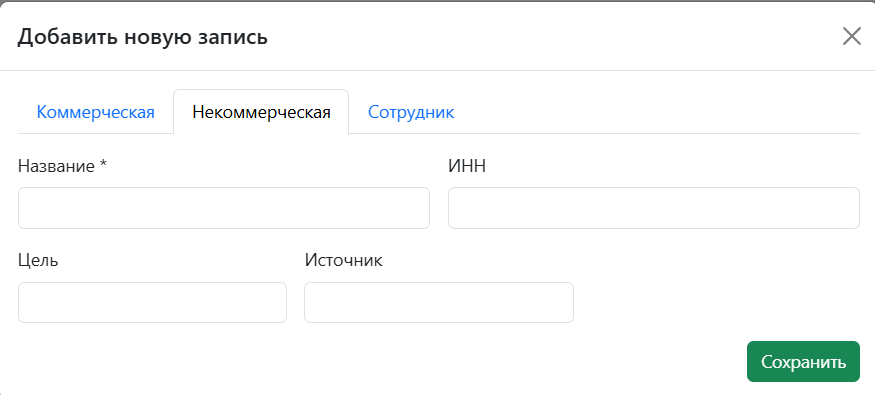
\includegraphics[width=0.8\textwidth]{добавление некоморг.png}
  \caption{Форма добавления некоммерческой организации}
  \label{fig:add_noncom}
\end{figure}


\begin{figure}[H]
  \centering
  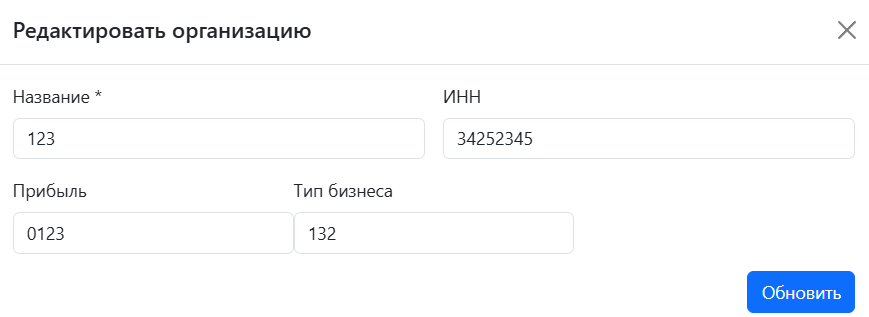
\includegraphics[width=0.8\textwidth]{редактирование комморг.png}
  \caption{Форма редактирования коммерческой организации}
  \label{fig:edit_com}
\end{figure}

\begin{figure}[H]
  \centering
  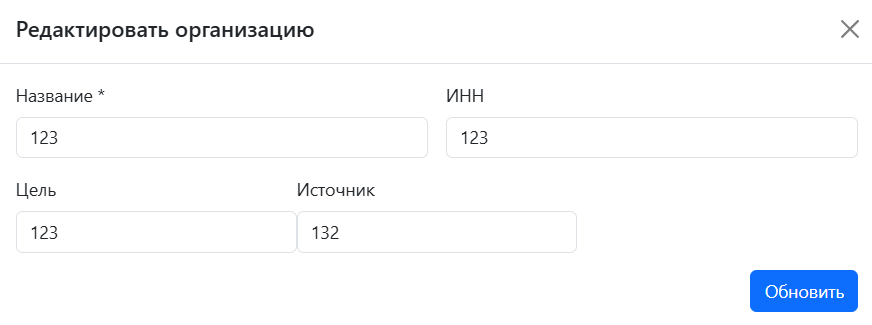
\includegraphics[width=0.8\textwidth]{редактирование некомморг.png}
  \caption{Форма редактирования некоммерческой организации}
  \label{fig:edit_noncom}
\end{figure}

\begin{figure}[H]
  \centering
  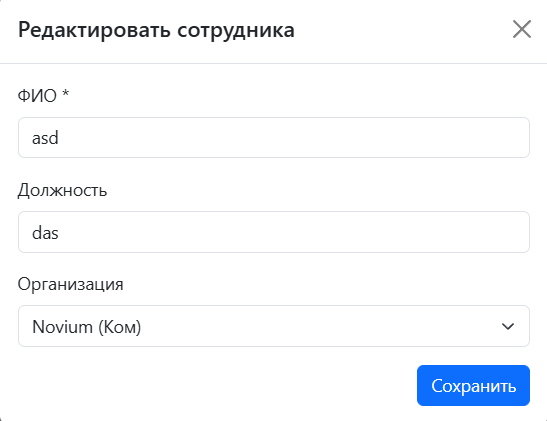
\includegraphics[width=0.8\textwidth]{редактирование сотрудника.png}
  \caption{Форма редактирования сотрудника}
  \label{fig:edit_emp}
\end{figure}

\newpage

\section*{Вывод}
\addcontentsline{toc}{section}{Вывод}

В ходе выполнения четвёртой лабораторной работы было успешно разработано распределённое веб-приложение с использованием двух языков: Go (сервер бизнес-логики и представления) и Python (сервер доступа к данным). Приложение демонстрирует современные подходы к проектированию микросервисных систем, чёткое разделение ответственности между слоями и эффективное применение объектно-ориентированного программирования. Реализованы все обязательные функции: CRUD через REST API, фильтрация и агрегация данных на стороне Go, кэширование с TTL 5 минут, бизнес-методы, а также удобный веб-интерфейс с валидацией и выпадающими списками.

\end{document}
